\chapter{Kontexters påverkan vid testning av GUI}
\chapterprecis{\LARGE{---- Olof Holmberg ----}}
\label{cha:indiv-report-holmberg}

\section{Inledning}
\label{sec:introduction-holmberg}

När man interagerar med mjukvara gör man det oftast genom ett grafiskt användargräns\-snitt. Då byggs en sekvens av interaktioner upp som bara blir längre och längre. Eftersom varje interaktion påverkar mjukvaran kan det uppstå fel som beror på hur denna sekvens är uppbyggd. Dessa fel behöver inte uppstå förrän sekvensen består av flera hundra olika interaktioner.

Kontexten är det som medför problem vid GUI-testning. Det är nästintill omöjligt att testa alla olika kombinationer av interaktioner som användarna kommer att utsätta mjukvaran för. Därför är det viktigt att vid test av GUI:t ta fram testfall som testar så många olika sekvenser som möjligt utan att testningen tar för lång tid. Den här utredningen undersöker hur man kan ta fram de sekvenser som är mest kritiska att testa samt hur det tillämpades på projektet.

\subsection{Syfte}
\label{sec:purpose-holmberg}

Syftet är att undersöka hur viktig kontexten för interaktioner är vid testning av GUI. Något som också undersöks är hur dessa testfall kan utformas för att inte få en testning som är alldeles för tids- och resurskrävande. Syftet är också att undersöka resultatet av att tillämpa testning som tar hänsyn till kontexten jämfört med testning som inte tar någon hänsyn till kontexter.

\subsection{Frågeställning}
\label{sec:issue-holmberg}

\begin{enumerate}
	\item Hur viktig är kontexten för interaktioner vid testning av GUI?
	\item Hur utformar man testfall som tar hänsyn till kontexten?
	\item Hade hänsyn till kontexter någon påverkan vid testning av 3DCopys GUI?
\end{enumerate}

\subsection{Avgränsningar}

Denna rapport fokuserar enbart på att undersöka testning av grafiska användargränssnitt där hänsyn har tagits till kontext. Denna begränsning tillämpas främst på de artiklar som har använts i denna rapport. Själva undersökningen är begränsad till en litteraturstudie samt resultatet av testningen som genomfördes på gruppens GUI.

\subsection{Definitioner, akronym och förkortningar}
Följande definitioner och förkortningar används på flera ställen i denna del av rapporten:
\begin{itemize}
	\item GUI (Graphical user interface) - Det grafiska användargränssnittet som används för att interagera med mjukvaran.
	\item Interaktion - När användaren av GUI:t interagerar med GUI:t genom att till exempel trycka på en knapp
	\item Kontext - Kontexten för en interaktion är sekvensen av interaktioner som har utförts på GUI:t innan den aktuella interaktionen.
\end{itemize}

\section{Bakgrund}
\label{sec:background-holmberg}

Ett av kraven för 3DCopy projektet var att det skulle finnas ett grafiskt användargränssnitt för mjukvaran som utvecklades. Då projektet ska utföras inom ett visst antal timmar måste man begränsa tiden som en uppgift får ta. Eftersom GUI testning kan ta i princip obegränsad tid så är det viktigt att hitta en gräns för när GUI testningen kan anses vara klar. Det är också viktigt att mjukvaran som kunden ska få är vältestad, därför är kontexter vid testning något som kan undersökas för att testa tillräckligt mycket på kort tid.

Som testledare är man ansvarig för alla tester som ska utföras på systemet och det känns därför relevant att undersöka detta område då det är en viktig del av projektet.

\section{Teori}
\label{sec:theory-holmberg}

Detta kapitel tar upp relevanta teoriaspekter om varför kontexten är viktig samt hur man kan utnyttja kontexten för att ta fram testfall.

\subsection{Vad är interaktionskontext?}

Kontexten för en interaktion är sekvensen av tidigare interaktioner med GUI:t. Till exempel för en interaktion i\textsubscript{i} är kontexten följande sekvens: <i\textsubscript{0}, i\textsubscript{1},  ... , i\textsubscript{i-1}>. Problemet som uppstår är att kontexten kan göras godtyckligt lång och att varje interaktion ska testas i alla möjliga kontexter. Det innebär att man kan testa ett GUI oändligt länge \cite{yuan2011gui}. 

\subsection{Betydelsen av kontext för interaktioner}

Enligt Yuan et al. \cite{yuan2011gui} är kontexten i vilken en interaktion med GUI:t utförs extremt viktigt och medför problem gällande testning av ett GUI. Kontexten kommer då att påverka framtida interaktioner och deras resultat. Ordningen av dessa interaktioner är essentiell för kontexten till en interaktion. För testning av ett GUI innebär detta att varje interaktion måste testas i flera kontexter. Till exempel kanske en viss interaktion genererar ett fel men enbart i en speciell kontext.

Så för att kunna identifiera fel är det framförallt tre saker som är viktigt. För det första är kontexten till en interaktion eller sekvens viktig, den kan vara avgörande för att hitta vissa fel. För det andra är positionen av interaktionerna i sekvensen viktig, det kan vara så att enbart en viss ordning av interaktioner triggar ett fel. För det tredje är ordningen som interaktionerna och sekvenserna testas i viktig då den påverkar vilka fel som hittas vid testning av GUI \cite{yuan2011gui}.

\subsection{Framtagning av testfall}
\label{sec:testcase-holmberg}

Den metod som föreslås av X. Yuan et al. \cite{yuan2011gui} innehåller följande steg:

\begin{itemize}
	\item [1] Generera EFG
	\item [2] Generera EIG
	\item [3] Välja styrka på testen
\end{itemize}

\subsubsection{Modellering av GUI}

Det första steget är att representera GUI:t som en event-flow-graph (EFG). En EFG representerar alla möjliga sekvenser av interaktioner som är möjliga att göra med GUI:t. Ett exempel på en EFG återfinns senare i rapporten i figur \ref{fig:3dcopy_guiefg}. Subvägarna i EFG:n representerar olika sekvenser av interaktioner. Men antalet subvägar i EFG:n ökar exponentiellt med längden på sekvensen. På grund av den exponentiella ökningen är det i princip omöjligt att kunna testa alla olika subvägar för sekvenser som består av fler än två interaktioner. För att minimera antalet noder i EFG:n gör man istället en event-interaktion-graph (EIG) \cite{yuan2011gui}. 

Andra steget är alltså att generera en EIG utifrån sin EFG. En EIG är en EFG utan noder (interaktioner) som inte påverkar mjukvaran bakom GUI:t, d.v.s. öppnandet av exempelvis menyer och fönster. Ett exempel på en EIG återfinns senare i rapporten i figur \ref{fig:3dcopy_guieig}. Metoden för att gå från en EFG till en EIG beskrivs av Xie och Memon \cite{xie2008using}. Metoden går ut på att man tar bort alla interaktioner som inte påverkar systemet med hjälp av regler för grafomskrivning \cite{yuan2011gui}. 

\subsection{Generering av testfall}

Första steget när man ska generera testfallen är att välja styrka. Styrkan kan vara två eller högre och säger hur många interaktioner som man är intresserad av. Till exempel skulle en styrka av två innebära att man väljer alla par av interaktioner från EIG:n som har en båge mellan sig. Eftersom att det är riktade bågar måste interaktionen som bågen utgår från vara först i paret. Dessa tupler som bildas efter man har valt styrkan utnyttjas sedan för att kunna ta fram kriterier för tillräcklighet hos testfallen \cite{yuan2011gui}. 

Det första som man vill uppnå med testfallen är tillräcklighet för något som kallas t-cover där t representerar styrkan. T-cover innebär att man i testfallen exekverar alla tupler av interaktioner som erhölls när man valde styrka på testfallen utan att andra interaktioner bryter den sekvensen \cite{yuan2011gui}.

Det andra man vill uppnå är t\textsuperscript{+}-cover. T\textsuperscript{+}-cover innebär att man exekverar tuplerna men med andra interaktioner mellan de som ingår i tupeln. När ett sådant test ingår för varje tupel är t\textsuperscript{+}-cover uppfyllt till 100 \% \cite{yuan2011gui}.

Enligt Yuan et al. \cite{yuan2011gui} om både t-cover och t\textsuperscript{+}-cover är uppfyllt anses testfallen vara t\textsuperscript{*}-cover. Det går även att utöka ytterligare med hjälp av arrayer men då ökar antalet testfall väldigt mycket och riskerar att ta för lång tid för att passa i projektets tidsplan. Därför kommer testerna enbart att uppfylla t\textsuperscript{*}-cover.

\section{Metod}
\label{sec:method-holmberg}

Först genomfördes en litteraturstudie för att samla information. Sedan testas 3DCopys GUI först med och sedan utan hänsyn till kontext för att se vilka fel som hittas av vilken testning. Dessa tekniker utvärderas sedan baserat på testresultatet.

\subsection{Testning av 3DCopys GUI med hänsyn till kontext}

Som test av GUI:t med hänsyn till kontext tas testfallen fram via den metod som presenteras i avsnitt \ref{sec:testcase-holmberg}.

\begin{figure}[H]
	\centering
	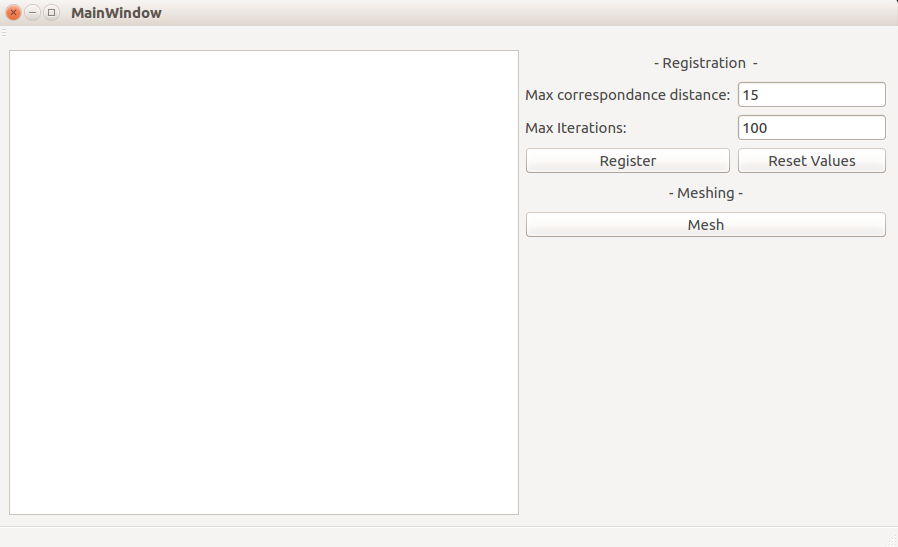
\includegraphics[width=130mm]{figures/3DCopyGUI.PNG}
	\caption{GUI:t för 3DCopy i slutet av iteration 2.}
	\label{fig:3dcopy_gui}
\end{figure}

GUI:t har 5 olika interaktioner som kan utföras. Man kan trycka på någon av de tre knapparna eller skriva i någon av de två input fälten. Det stora vita fältet är till för att visa meddelanden från mjukvaran och kan ej interageras med. Utifrån dessa 5 interaktioner kan vi ta fram EFG:n för GUI:t.

\begin{figure}[H]
	\centering
	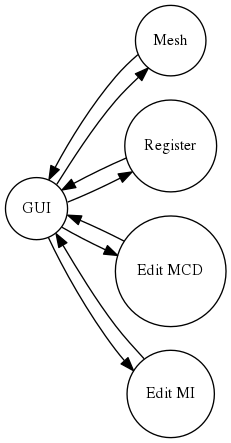
\includegraphics[width=50mm]{figures/3DCopyGUIEFG.png}
	\caption{EFG:n för 3DCopys GUI.}
	\label{fig:3dcopy_guiefg}
\end{figure}

Utifrån EFG:n ska sedan EIG:n skapas. Det som händer vid skapandet av EIG:n är att noderna GUI, Edit MCD och Edit MI tas bort eftersom att de inte interagerar med systemet.

\begin{figure}[H]
	\centering
	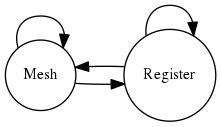
\includegraphics[width=50mm]{figures/3DCopyGUIEIG.png}
	\caption{EIG:n för 3DCopys GUI.}
	\label{fig:3dcopy_guieig}
\end{figure}

Nu när EIG:n är framtagen ska styrka väljas på testen. För att testerna ska skilja sig lite mer från de testerna utan hänsyn till kontext men åndå inte ta för lång tid väljs styrka 3 på dessa tester. Det innebär att vi får följande sekvenser som ska användas för att ta fram testfallen.

\begin{table}[h]
	\caption{De sekvenser som ska användas för att ta fram testfallen.}
	\label{tbl:test_seq}
	\centering
\begin{tabular}{|l|l|}
	\hline
	\textbf{Nr} & \textbf{Sekvens} \\
	\hline
	1 & <Mesh, Mesh, Mesh> \\
	\hline
	2 & <Mesh, Mesh, Register> \\
	\hline
	3 & <Mesh, Register, Mesh> \\
	\hline
	4 & <Mesh, Register, Register> \\
	\hline
	5 & <Register, Mesh, Mesh> \\
	\hline
	6 & <Register, Mesh, Register> \\
	\hline
	7 & <Register, Register, Mesh> \\
	\hline
	8 & <Register, Register, Register> \\
	\hline
\end{tabular}
\end{table}

Dessa sekvenser kombineras sedan för att testfallen ska uppnå 3-cover och 3\textsuperscript{+}-cover och därför också 3\textsuperscript{*}-cover. Först genererades två stycken olika  mängder med testfall som enskilt uppfyllde antingen 3-cover eller 3\textsuperscript{+}-cover. Dessa kombinerades sedan för att få fram den mängd testfall som ska utföras på GUI:t.

\begin{table}[h]
	\caption{De testfall genomfördes på GUI:t med hänsyn till kontext.}
	\label{tbl:test_context}
	\centering
	\begin{tabular}{|l|l|}
		\hline
		\textbf{Nr} & \textbf{Testfall} \\
		\hline
		1 & <Register, Mesh, Register, Mesh, Register, Mesh> \\
		\hline
		2 & <Mesh, Register, Mesh, Register, Mesh, Register> \\
		\hline
		3 & <Register, Mesh, Mesh, Mesh, Register, Mesh> \\
		\hline
		4 & <Mesh, Mesh, Register, Register, Register, Mesh> \\
		\hline
		5 & <Mesh, Mesh, Register, Mesh, Register, Mesh> \\
		\hline
		6 & <Register, Mesh, Mesh, Register, Mesh, Register> \\
		\hline
		7 & <Register, Mesh, Register, Register, Register, Mesh> \\
		\hline
		8 & <Mesh, Register, Register, Mesh, Mesh, Register> \\
		\hline
		9 & <Mesh, Register, Register, Mesh, Register, Mesh> \\
		\hline
		10 & <Mesh, Register, Mesh, Register, Register, Mesh> \\
		\hline
		11 & <Register, Mesh, Mesh, Register, Register, Mesh> \\
		\hline
		12 & <Register, Register, Mesh, Register, Mesh, Register> \\
		\hline
	\end{tabular}
\end{table}

GUI:t testas sedan genom att utföra dessa testfall i den ordning som visas i tabell \ref{tbl:test_context}. GUI:t startades om mellan varje testfall. Dessa tester utfördes manuellt på GUI:t.

\subsection{Testning av 3DCopys GUI utan hänsyn till kontext}

Som test av GUI:t utan hänsyn till kontext kan man tänka sig att en så kallad full-branch coverage kan vara tillräcklig. Det vill säga att alla olika vägar som man kan gå i GUI:t testas. Det blir alltså totalt N! antal test där N är antalet interaktioner som kan utföras på GUI:t.

\begin{table}[h]
	\caption{De testfall som genomfördes på GUI:t utan hänsyn till kontext.}
	\label{tbl:test_nocontext}
	\centering
	\begin{tabular}{|l|l|}
		\hline
		\textbf{Nr} & \textbf{Testfall} \\
		\hline
		1 & <Register, Mesh> \\
		\hline
		2 & <Mesh, Register> \\
		\hline
	\end{tabular}
\end{table}

GUI:t testas sedan genom att utföra dessa testfall i den ordning som visas i tabell \ref{tbl:test_nocontext}. GUI:t startas om mellan varje testfall. Dessa tester utfördes manuellt på GUI:t.

\section{Resultat}
\label{sec:results-holmberg}

Här presenteras de resultat som erhölls från både litteraturstudien och de tester som genomfördes på GUI:t.

Litteraturstudien visar ett tydligt samband mellan kontexten och vilka fel som testerna lyckas hitta. Kontexten är alltså avgörande för hur interaktionen kommer att påverka mjukvaran \cite{yuan2011gui}. 

\subsection{Testresultat}

I detta avsnitt presenteras de resultat som erhölls vid den testning av GUI:t som genomfördes.

\subsubsection{Med hänsyn till kontext}

Testfallen med hänsyn till kontext lyckades identifiera ett fel i meshningen. Den klarar bara av att mesha en viss fil, \textit{first\_registered\_church.pcd}. Eftersom att den tar lång tid att mesha utfördes enbart test nummer ett i tabell \ref{tbl:test_context} med denna fil. Resterande tester utfördes med andra filer som fick fel i meshningen. Alltså exekverades inte meshningskoden i de flesta fall utan bara tills felet uppstod.

\subsubsection{Utan hänsyn till kontext}

De tester som utfördes utan hänsyn till kontext hittade samma fel som de med hänsyn till kontext. Alltså att meshningen enbart klarade av en av filerna. Dessa tester utfördes båda med filer som klarade eller fick fel i meshningen.

\section{Diskussion}
\label{sec:discussion-holmberg}

I detta avsnitt diskuteras resultatet, den metod som användes samt källkritik.

\subsection{Resultat}

Som resultatet visar lyckades de båda testen identifiera samma fel trots att det med hänsyn till kontext var mycket mer omfattande. Och detta resultat kan bero på många olika saker. Dels hade systemet som testades enbart två systeminteraktioner och dessa två använder ingen delad kod. Därför är sannolikheten för att de påverkar något i koden som förstör för den andra interaktionen väldigt liten.

Dessa interaktioner är också testade sedan tidigare i andra systemtest och därför kan alla fel i koden redan vara lösta. Så sannolikheten för att det skulle finnas något fel kvar minskar ytterligare. Så det resultat som erhölls är ganska sannolikt med tanke på omständigheterna. Hade systemet varit större med fler interaktioner som delvis använder samma kod hade testningen med hänsyn till kontext eventuellt hittat fler fel.

\subsection{Metod}

En stor brist i litteraturstudien är avsaknaden av ytterligare källor. "Kontext", i kombination med testningsrelaterade termer, var de sökord som användes under sökandet av ytterligare källor. Det hade eventuellt varit fördelaktigt att utforska andra termer som beskriver kontext då inga ytterligare relevanta källor hittades. Att söka efter andra termer var dock något som inte genomfördes på grund av tidsbrist.

Den främsta bristen i metoden är att felet i meshningen inte hade hittats och blivit löst innan dessa tester. Eftersom att den enda filen som kunde meshas tog väldigt lång tid var det inte realistiskt att genomföra alla tester med den och därför är inte alla testfall med hänsyn till kontext genomförda med den filen. Det medför i sin tur att de testerna aldrig exekverade koden som utför meshningen och det kan därför finnas kontextkänsliga fel i den biten av koden som inte hittades.

Den kontextkänsliga testningen begränsades också vid t\textsuperscript{*}-cover. Det finns ytterligare ett steg som är ännu kraftfullare som kanske skulle ha hittat fel som inte identifierades.

Den kontextkänsliga testningen borde också jämförts med en annan GUI testnings metod, inte bara en testning som uppnår full path coverage. Detta för att kunna jämföra olika GUI testnings metoder.

\subsection{Källkritik}

För litteraturstudien hittades bara en relevant artikel som berörde den bit som var mest kritisk för att utföra testerna, nämligen en som tog upp hur man testar GUI:n med hänsyn till kontext. Den artikeln är skriven av personer med lång erfarenhet inom just GUI testning vilket framgick när sökandet efter ytterligare artiklar genomfördes eftersom många artiklar som dök upp var skrivna av samma personer. En anledning  till att det var svårt att hitta ytterligare artiklar kan vara att Yuan et al. \cite{yuan2011gui} har valt att kalla det för kontext. Då de också definierar begreppet kontext i sin artikel indikerar det att de eventuellt är en av få eller den enda artikeln inom just detta ämne. Eller så har andra artiklar valt en annan benämning än just kontext.

\section{Slutsatser}
\label{sec:conclusions-holmberg}

Att ta hänsyn till kontexten vid GUI testning är definitivt något som bör göras. Den är ofta avgörande för att hitta vissa fel. Det hade varit intressant att skapa exempel GUI:n med medvetet placerade fel som beror på andra interaktioner för att kunna undersöka detta noggrannare. Det fanns dock inte tid att göra en sådan undersökning i denna rapport. Därför får betydelsen av kontexter begränsas till litteraturstudien.

Gällande metoden för att ta fram testfall med hänsyn till kontext användes samma metod som i Yuan et al. \cite{yuan2011gui}. Något som blev tydligt då testerna utfördes manuellt är att metoden inte tar hänsyn till hur resurs- eller tidskrävande en interaktion är när man placerar den i sekvensen. Det är något som man skulle kunna bygga vidare på. Att undersöka hur de mest krävande interaktionerna ska placeras i sekvenserna för att testa så många kontexter som möjligt och samtidigt minimera tids- och resurskostnader.

Testerna visade att för projektets GUI, i det stadie som GUI:t befann sig i vid testningen, spelade inte kontexten någon roll för att hitta fel. Det beror sannolikt på att mängden interaktioner var liten samt att systeminteraktionerna var väl separerade och inte delade någon kod. Det indikerar att hänsyn till kontexten blir viktigare ju större mängd interaktioner GUI:t har samt hur stor del av koden som interaktionerna har gemensamt. Hade mer tid funnits skulle en undersökning med olika GUI:n med varierande antal interaktioner varit intressant för att vidare kunna undersöka denna teori.

%%%%%%%%%%%%%%%%%%%%%%%%%%%%%%%%%%%%%%%%%%%%%%%%%%%%%%%%%%%%%%%%%%%%%%
%%% holmberg-report.tex ends here
